
\section{夜の座談会}
\subsection{日時・場所}
日時:2019年4月5日(金) 20:00 $\sim$ \ (入浴が終わった人から順に参加) \\
\ \ \ 場所:食堂・ロビー\\

\subsection{目的}
一年生が先輩との交流を深め,学校生活で心配なことなどを聞く.
\subsection{イベント内容(概要)}
ロビーでカードゲームやボードゲームを,食堂内でブースを4つ(履修・授業ブース,フリー,サークル,バイト)用意し自由に一年生が回る.食堂では,一つのブースに
テーマに沿ったテンプレのような用紙を用意しておく

\subsection{タイムスケジュール}
\begin{longtable}{p{3zw}p{39zw}}
  20:00 & \textbf{◎ 夜の座談会開始}\\
        &  \ \ \textbullet \ \ 新一年生には順次参加してもらう\\\\
        
  21:30 & \textbf{◎ 終了}
\end{longtable}

\subsection{必要物品}
\begin{itemize}
\item ブースのテーマ用紙:12枚
\item トークテーマ用紙:30枚
\item トランプ:2つ,UNO:1つ
\item オリジナルすごろく(ボートゲーム):2つ,サイコロ:3つ
\item お菓子:いっぱい
\item 飲み物:ジュースをいっぱい
\item 紙皿
\item 紙コップ
\item 割り箸
\item サインペン
\item ウェットティッシュ:5個
\item キッチンペーパー:6個
\item ゴミ袋:6個
\end{itemize}

\subsection{人員配置}
\begin{itemize}
\item 勉強:塩谷
\item サークル:中島
\item バイト:北村
\item フリートーク:吉田
\item ゲーム:高橋(龍),丸田
\item その他;角原,小松,渡辺,小谷,斎藤,藤田(B3),立岩,日下,堀川
\end{itemize}

\subsection{備考}
\begin{itemize}
\item トランプは堀川と藤沢, UNOは藤沢が持ってくる
\item 座談会は教授も参加OK
\end{itemize}

\subsection{全体配置}
\begin{center}
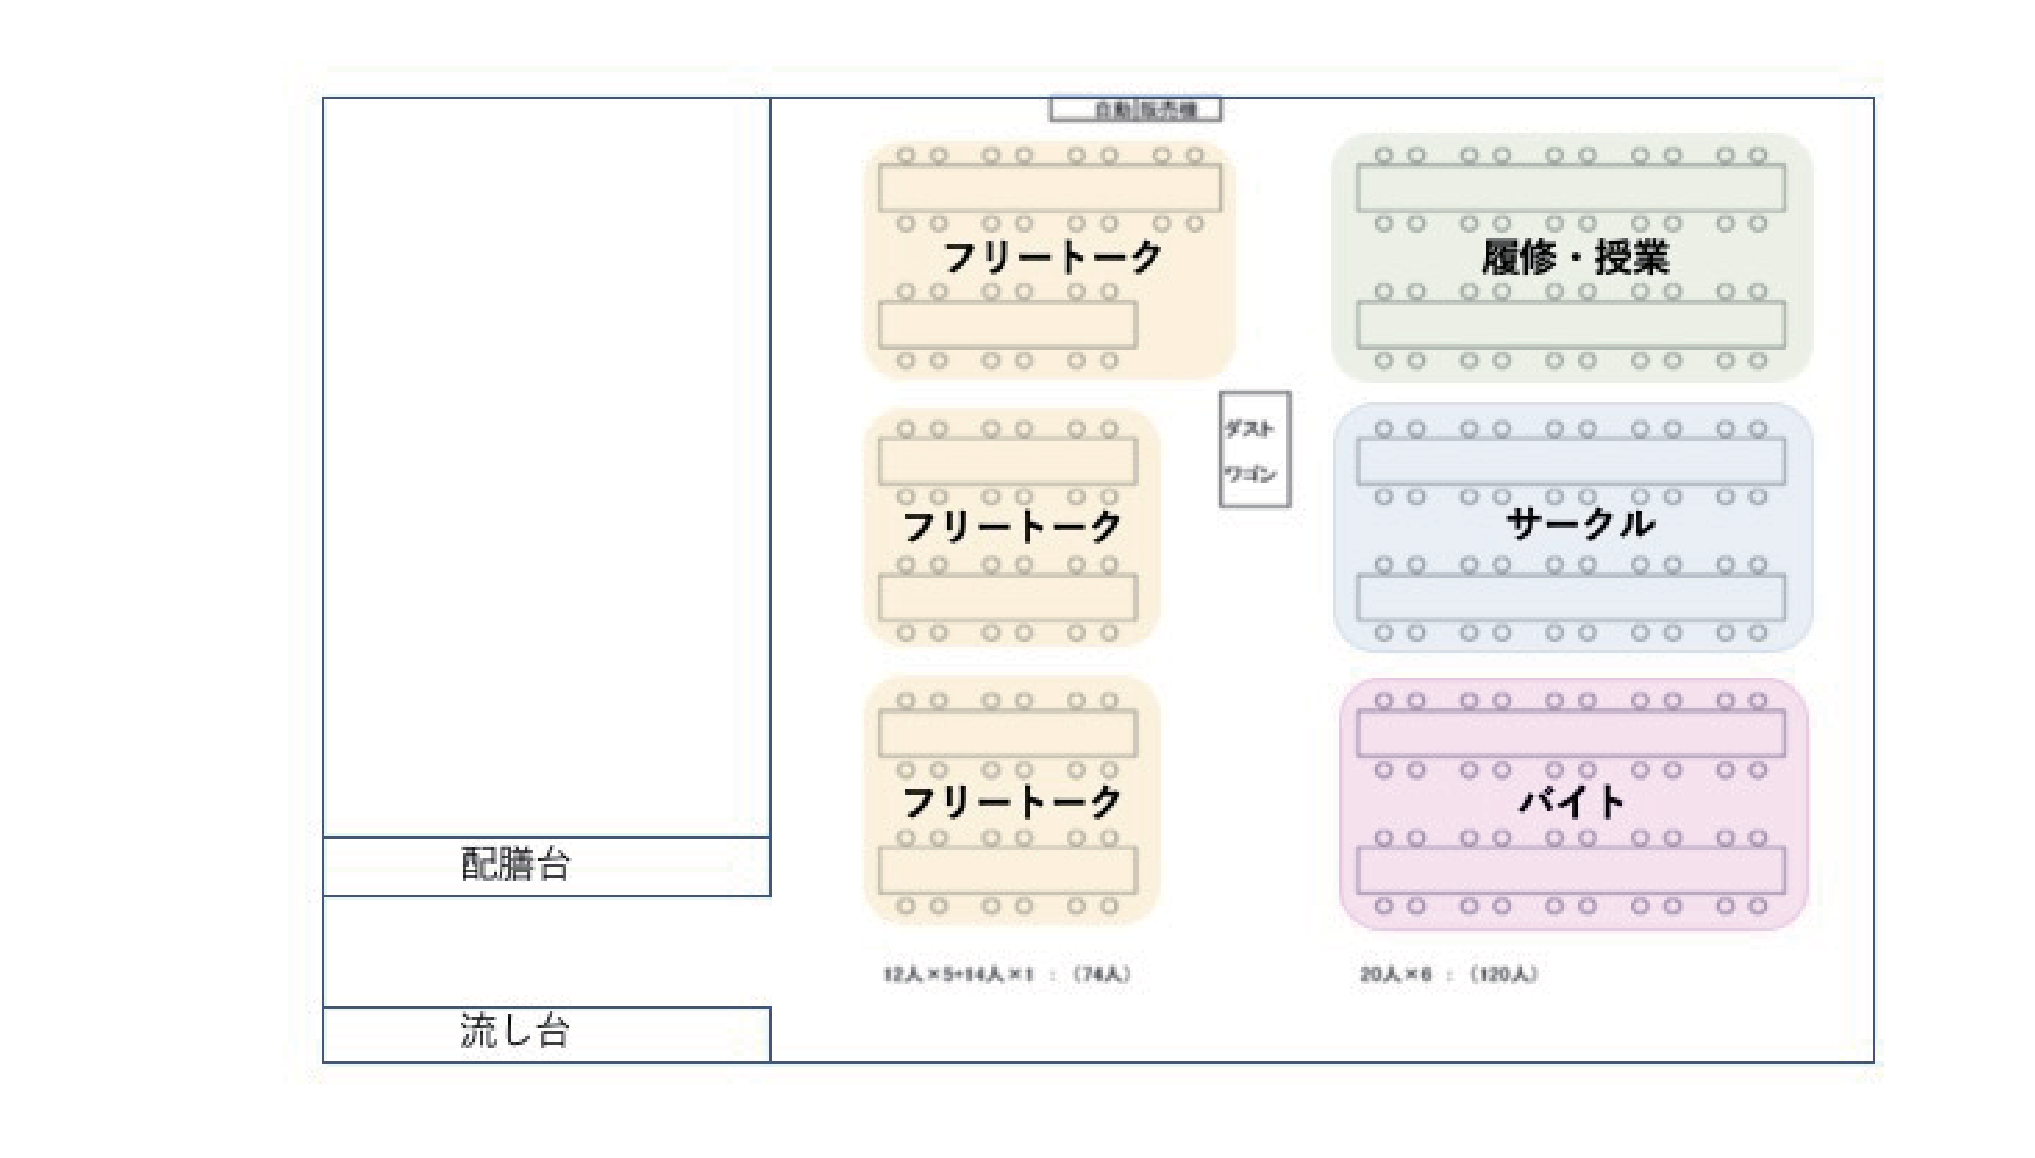
\includegraphics[width=15cm]{./13/hone.eps}
\end{center}
